\documentclass{beamer}

\usepackage[utf8]{inputenc}
\usepackage{tikz}
\usepackage{hyperref}
\usepackage{listings}
\usepackage{float}

\lstset{language=SQL,morekeywords={RETURN,FOREACH},
  columns=flexible,showstringspaces=false, framexleftmargin=15pt}

\usetikzlibrary{positioning,shapes,arrows}

\usetheme{Madrid}

\title{Neo4j}

\author{David Antuña \and Daniel Gutiérrez}

\institute[UCM]
{
  Bases de Datos NoSQL\\
  Universidad Complutense de Madrid
}

\date{Curso 2017-18}

\subject{Introduction to Neo4j}

\pgfdeclareimage[height=0.5cm]{university-logo}{images_ignore/university-logo-filename}
\logo{\pgfuseimage{university-logo}}

\AtBeginSubsection[]
{
  \begin{frame}<beamer>{Contenidos}
    \tableofcontents[currentsection,currentsubsection]
  \end{frame}
}

\begin{document}

\begin{frame}
	\titlepage
\end{frame}

\begin{frame}{Contenidos}
	\tableofcontents
\end{frame}

% Section and subsections will appear in the presentation overview
% and table of contents.
\section{Introducción}

\begin{frame}{Introducción}
	\begin{itemize}
		\item Transaccional
		      \begin{itemize}
			      \item Full ACID (Atomicity, Consistency, Isolation, Durability)
		      \end{itemize}
		\item Orientada a Grafos
		\item Implementada en Java
		\item Cypher
		\item Schema-less
		\item Limitado a
		      \begin{itemize}
			      \item 32x$10^9$ nodos
			      \item 32x$10^9$ relaciones
		      \end{itemize}
	\end{itemize}
\end{frame}

\subsection{Ventajas}

\begin{frame}{Ventajas}
	\begin{itemize}
		\item Rendimiento
		      \pause
		\item Flexibilidad
		\item Escalabilidad
		      \pause
    \item Interfaz gráfica
	\end{itemize}
\end{frame}

\subsection{Desventajas}

\begin{frame}{Desventajas}
	\begin{itemize}
		\item Limitaciones al tamaño de la base
		      \pause
		\item No Sharding
	\end{itemize}
\end{frame}

\section{Cypher}

\subsection{¿Qué es?}

\begin{frame}{¿Qué es?}
	\begin{itemize}
		\item Lenguaje declarativo
		      \pause
		\item Inspirado en SQL
		      \pause
		\item Visual
		      \pause
	\end{itemize}

	\begin{block}{Ejemplo}
		\begin{center}
			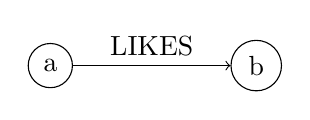
\begin{tikzpicture}
				\node [circle, draw=black] (a) {a};
				\node [circle, draw=black, right=2 of a] (b) {b};

				\path[->]
				(a.east)
				edge node[above] {LIKES} (b);
			\end{tikzpicture}

			\vspace{5mm}
			(a)~~-[:LIKES]-$>$~~(b)
		\end{center}

	\end{block}
\end{frame}

\subsection{Nodos}

\begin{frame}{Nodos}
	\begin{itemize}
		\item Delimitados por paréntesis
		      \pause
		\item Se pueden asignar variables
		      \pause
	\end{itemize}


	\begin{block}{Ejemplo 1}
		MATCH (p:Person) RETURN p.name
	\end{block}
	\pause
	\begin{block}{Ejemplo 2}
		MATCH (p:Person)\\
		WHERE p.name STARTS WITH $'$T$'$\\
		RETURN p.name as name
	\end{block}
\end{frame}

\subsection{Relaciones}

\begin{frame}{Relaciones}
	\begin{itemize}
		\item Flechas, - -$>$, entre dos nodos
		      \pause
		\item Permiten especificar informacion entre corchetes
		      \pause
		      \begin{itemize}
			      \item Tipo ~~~-[:LIKES$\mid$:KNOWS]-$>$
			            \pause
			      \item Variable~~~-[rel:LIKES]-$>$
			            \pause
			      \item Propiedades~~~-[\{since:2010\}]-$>$
			            \pause
			      \item Longitud máxima~~~-[:KNOWS*..4]-$>$
			            \pause
		      \end{itemize}
	\end{itemize}


	\begin{block}{Ejemplo}
		MATCH (actor:Person)~~-[:ACTED\_IN]-$>$~~(movie:Movie)\\
		WHERE movie.title STARTS WITH $'$Avengers$'$\\
		RETURN movie.title as title
	\end{block}
\end{frame}

\subsection{Patrones}

\begin{frame}{Patrones}
	\begin{itemize}
		\item Se construyen mediante nodos y relaciones
		\item Pueden ir seguidos o separados por comas
	\end{itemize}
	\pause
	\vspace{2mm}
	\begin{itemize}
		\item Amigo de un amigo\\
		      {\scriptsize(user)-[:KNOWS]-(friend)-[:KNOWS]-(foaf)}\\
		      \pause
		      {\scriptsize(user)-[:KNOWS]-(friend), (friend)-[:KNOWS]-(foaf)}
		      \pause
		\item Camino mínimo\\
		      {\scriptsize path = shortestPath( (user)-[:KNOWS*..5]-(other) )}
		      \pause
		\item Filtrado colaborativo\\
		      {\scriptsize(user)-[:BOUGHT]-$>$(product)$<$-[:BOUGHT]-()-[:BOUGHT]-$>$(otherProduct)}
		      \pause
		\item Navegación en árbol\\
		      {\scriptsize(root)$<$-[:PARENT*]-(leaf:Category)-[:ITEM]-$>$(data:Product)}
	\end{itemize}
\end{frame}

\section{Ejemplo}

\begin{frame}{Ejemplo}
	\lstinputlisting{example/example1.sql}
\end{frame}

\begin{frame}{Ejemplo}
	\lstinputlisting{example/example2.sql}
\end{frame}

\appendix
\section<presentation>*{\appendixname}
\subsection<presentation>*{Referencias}

\begin{frame}[allowframebreaks]
	\frametitle<presentation>{Referencias}

	\begin{thebibliography}{9}

		\setbeamertemplate{bibliography item}[online]

		\bibitem{A}
		{\em \href{https://neo4j.com/graphacademy/}{Neo4j}}

		\bibitem{B}
		{\em \href{https://bbvaopen4u.com/es/actualidad/neo4j-que-es-y-para-que-sirve-una-base-de-datos-orientada-grafos}{BBVA - Ventajas Neo4j}}

		\bibitem{C}
		{\em \href{https://neo4j.com/developer/cypher-query-language/}{Cypher}}

		\bibitem{D}
		{\em \href{https://neo4j.com/docs/cypher-refcard/current/}{Refcard Cypher}}

	\end{thebibliography}
\end{frame}

\end{document}
